\usepackage{tikz}

\counterwithout{figure}{section}
\counterwithout{table}{section}
\counterwithout{equation}{section}

\titleformat{\subsection}[block]
  {\bfseries\filcenter}{#1}{0cm}{}
\titlespacing{\subsection}{0cm}{21pt}{21pt}

\DeclareCaptionLabelFormat{gosttable}{Таблица #2}

\usepackage{float}
\usepackage{pgfplots}
\usepackage{graphicx}
\usepackage{multirow}
\usepackage{amssymb,amsfonts,amsmath,amsthm}

\usepackage{listings}
\lstset{basicstyle=\footnotesize\ttfamily,breaklines=true}
\lstset{language=Matlab}


\newcommand{\labnumber}{5} % fifth lab
\usepackage{tikz}

\counterwithout{figure}{section}
\counterwithout{table}{section}
\counterwithout{equation}{section}

\titleformat{\subsection}[block]
  {\bfseries\filcenter}{#1}{0cm}{}
\titlespacing{\subsection}{0cm}{21pt}{21pt}

\DeclareCaptionLabelFormat{gosttable}{Таблица #2}

\newcommand{\khpistudentgroup}{2.КН201н.8а}
\newcommand{\khpistudentname}{Чепурний~А.~С.}

\newcommand{\khpidepartment}{Програмна інженерія та інформаційні технології управління}
\newcommand{\khpititlewhat}{
	Розрахунково-графічне завдання \\
	з предмету <<Фреймворки та платформи>>
}
\newcommand{\khpititlewho}{
	Виконав: \\
	\hspace*{\parindent} ст. групи \khpistudentgroup \\
	\hspace*{\parindent} \khpistudentname \\
	Перевірила: \\
	\hspace*{\parindent} к. т. н., вик. каф. ПІІТУ \\
	\hspace*{\parindent} Добряк~В.~С. \\
}


\usepackage{systeme}
\usepackage{longtable,tabu}
\usepackage{multirow}
\usepackage{array,multirow}
\usepackage{pdflscape}
\usepackage{afterpage}
\usepackage{tikz}
\usepackage{bm}

\graphicspath{{figures/}}

\begin{document}
\Russian

\begin{titlepage}

\begin{center}
	МІНІСТЕРСТВО ОСВІТИ І НАУКИ УКРАЇНИ \\
	НАЦІОНАЛЬНИЙ ТЕХНІЧНИЙ УНІВЕРСИТЕТ \\
	«ХАРКІВСЬКИЙ ПОЛІТЕХНІЧНИЙ ІНСТИТУТ» \\
	Кафедра <<\khpidepartment>> \\
\end{center}

\vspace{6cm}

\begin{center}
	\khpititlewhat
\end{center}

\vspace{3cm}

\begin{addmargin}[10cm]{0cm}
	\khpititlewho
\end{addmargin}

\vspace{\fill}

\begin{center}
	Харків \the\year
\end{center}

\end{titlepage}

\addtocounter{page}{1}

\textbf{Тема}: операции над нечеткими числами на основе принципа обобщения.

\textbf{Цель}: 
\begin{itemize}
	\item изучить теоретические основы по выполнению арифметических операций над нечеткими числами (сложение, вычитание, умножение, деление);
	\item закрепить теоретические знания решением практической задачи;
	\item провести анализ полученных результатов и сделать выводы по работе.
\end{itemize}

\textbf{Задание}: 
\begin{itemize}
	\item выполнить арифметическую операцию \textit{СЛОЖЕНИЯ} над двумя нечеткими числами $\tilde{N}$ и $\tilde{M}$, то есть $\tilde{N}+\tilde{M}$;
	\item выполнить арифметическую операцию \textit{ВЫЧИТАНИЯ} над двумя нечеткими числами $\tilde{N}$ и $\tilde{M}$, то есть $\tilde{N}-\tilde{M}$;
	\item выполнить арифметическую операцию \textit{УМНОЖЕНИЯ} над двумя нечеткими числами $\tilde{N}$ и $\tilde{M}$, то есть $\tilde{N} \times \tilde{M}$;
	\item выполнить арифметическую операцию \textit{ДЕЛЕНИЯ} над двумя нечеткими числами $\tilde{N}$ и $\tilde{M}$, то есть $\tilde{N} \div \tilde{M}$;
\end{itemize}

Для каждого действия представить геометрическую интерпретацию исходных данных и результата.

Провести анализ полученных результатов.

\textbf{Исходные данные}: 

Нечеткой величиной называется произвольное нечеткое множество $\tilde{A} = \{x, \mu_{\tilde{A}} (x)\}$. 
Пусть $\tilde{N} = \tilde{2} = \{ <0.6, 1>, <1.0, 2>, <0.8, 3> \}$ и $\tilde{M} = \tilde{2} = \{ <0.8, 5>, <1.0, 6>, <0.7, 7> \}$ (рисунок~\ref{fig:source}).

\begin{figure}[H]
    \centering
    \begin{subfigure}[b]{0.35\textwidth}
		\centering
		\begin{tikzpicture}[scale=0.6]
			\begin{axis}[
			  ymin=0,
			  xlabel=$x$,
			  ylabel=$y$,]
			  \addplot coordinates {(1,0.6) (2,1) (3,0.8)};
			\end{axis}
		\end{tikzpicture}
        \caption{Геометрическая интерпретация $\tilde{N}$}
        \label{fig:n}
    \end{subfigure}
    ~
    \begin{subfigure}[b]{0.35\textwidth}
		\centering
		\begin{tikzpicture}[scale=0.6]
			\begin{axis}[
			  ymin=0,
			  xlabel=$x$,
			  ylabel=$y$,]
			  \addplot coordinates {(5,0.8) (6,1) (7,0.7)};
			\end{axis}
		\end{tikzpicture}
        \caption{Геометрическая интерпретация $\tilde{M}$}
        \label{fig:m}
    \end{subfigure}
	\caption{Геометрическая интерпретация исходных данных}
	\label{fig:source}
\end{figure}

\subsection{Сложение нечетких чисел}
Операция сложения нечетких чисел (интервалов) обозначается через $\tilde{N}+\tilde{M} = \tilde{O} = \{ z, \mu_{\tilde{O}} (z) \}$, где функция принадлежности результата $\mu_{\tilde{O}} (z)$ определяется по формуле:
\[
	\mu_{\tilde{O}} (z) = \sup_{z=x+y} \{ \min \{ \mu_{\tilde{N}} (x), \mu_{\tilde{M}} (y) \} \}.
\]

Получим: 
\begin{multline*}
	\tilde{O} = \tilde{N} + \tilde{M} = \{ <0.6, 1>, <1.0, 2>, <0.8, 3> \} + \\
	+ \{ <0.8, 5>, <1.0, 6>, <0.7, 7> \} = \\ 
	= \{ 
		<\min \{ 0.6, 0.8 \}, 6>, \\
		<\max\{ \min \{ 0.6, 1.0 \}, \min \{ 1.0, 0.8 \}, \}, 7>, \\
		<\max\{ \min \{ 0.6, 0.7 \}, \min \{ 1.0, 1.0 \}, \min \{ 0.8, 0.8 \}, \}, 8>, \\
		<\max\{ \min \{ 1.0, 0.7 \}, \min \{ 0.8, 1.0 \}, \}, 9>, \\
		<\min \{ 0.8, 0.7 \}, 10> \} = \\
		= \{ < 0.6, 6 >, < 0.8, 7 >, < 1.0, 8 >, < 0.8, 9 >, < 0.7, 10 > \}.
\end{multline*}

Графическая интерпретация представлена на рисунке~\ref{fig:n_plus_m}.

\begin{figure}[H]
    \centering
	\begin{tikzpicture}
		\begin{axis}[
		  ymin=0,
		  xlabel=$x$,
		  ylabel=$y$,]
		  \addplot coordinates {(6,0.6) (7,0.8) (8,1.0) (9,0.8) (10,0.7)};
		\end{axis}
	\end{tikzpicture}
    \caption{Геометрическая интерпретация $\tilde{O}=\tilde{N} + \tilde{M}$}
    \label{fig:n_plus_m}
\end{figure}

\subsection{Вычитание нечетких чисел}
Операция вычитания нечетких чисел (интервалов) обозначается через $\tilde{N}-\tilde{M} = \tilde{O} = \{ z, \mu_{\tilde{O}} (z) \}$, где функция принадлежности результата $\mu_{\tilde{O}} (z)$ определяется по формуле:
\[
	\mu_{\tilde{O}} (z) = \sup_{z=x-y} \{ \min \{ \mu_{\tilde{N}} (x), \mu_{\tilde{M}} (y) \} \}.
\]

Получим: 
\begin{multline*}
	\tilde{O} = \tilde{N} - \tilde{M} = \{ <0.6, 1>, <1.0, 2>, <0.8, 3> \} - \\
	- \{ <0.8, 5>, <1.0, 6>, <0.7, 7> \} = \\ 
	= \{ < 0.6, -6 >, < 0.7, -5 >, < 1.0, -4 >, < 0.8, -3 >, < 0.8, -2 > \}
\end{multline*}

Графическая интерпретация представлена на рисунке~\ref{fig:n_minus_m}.

\begin{figure}[H]
    \centering
	\begin{tikzpicture}
		\begin{axis}[
		  ymin=0,
		  xlabel=$x$,
		  ylabel=$y$,]
		  \addplot coordinates {(-6,0.6) (-5,0.7) (-4,1.0) (-3,0.8) (-2,0.8)};
		\end{axis}
	\end{tikzpicture}
    \caption{Геометрическая интерпретация $\tilde{O}=\tilde{N} - \tilde{M}$}
    \label{fig:n_minus_m}
\end{figure}

\subsection{Умножение нечетких чисел}
Операция умножения нечетких чисел (интервалов) обозначается через $\tilde{N} \times \tilde{M} = \tilde{O} = \{ z, \mu_{\tilde{O}} (z) \}$, где функция принадлежности результата $\mu_{\tilde{O}} (z)$ определяется по формуле:
\[
	\mu_{\tilde{O}} (z) = \sup_{z=x \times y} \{ \min \{ \mu_{\tilde{N}} (x), \mu_{\tilde{M}} (y) \} \}.
\]

Получим: 
\begin{multline*}
	\tilde{O} = \tilde{N} \times \tilde{M} = \{ <0.6, 1>, <1.0, 2>, <0.8, 3> \} \times \\
	\times \{ <0.8, 5>, <1.0, 6>, <0.7, 7> \} = \\ 
	= \{ < 0.6, 5 >, < 0.6, 6 >, < 0.6, 7 >, < 0.8, 10 >, \\ < 1.0, 12 >, < 0.7, 14 >, < 0.8, 15 >, < 0.8, 18 >, < 0.7, 21 > \}.
\end{multline*}

Графическая интерпретация представлена на рисунке~\ref{fig:n_by_m}.

\begin{figure}[H]
    \centering
	\begin{tikzpicture}
		\begin{axis}[
		  ymin=0,
		  xlabel=$x$,
		  ylabel=$y$,]
		  \addplot coordinates {(5,0.6) (6,0.6) (7,0.6) (10,0.8) (12,1.0) (14,0.7) (15,0.8) (18,0.8) (21,0.7)};
		\end{axis}
	\end{tikzpicture}
    \caption{Геометрическая интерпретация $\tilde{O}=\tilde{N} \times \tilde{M}$}
    \label{fig:n_by_m}
\end{figure}

\subsection{Деление нечетких чисел}
Операция деления нечетких чисел (интервалов) обозначается через $\tilde{N} \div \tilde{M} = \tilde{O} = \{ z, \mu_{\tilde{O}} (z) \}$, где функция принадлежности результата $\mu_{\tilde{O}} (z)$ определяется по формуле:
\[
	\mu_{\tilde{O}} (z) = \sup_{z=x \div y} \{ \min \{ \mu_{\tilde{N}} (x), \mu_{\tilde{M}} (y) \} \}.
\]

Получим: 
\begin{multline*}
	\tilde{O} = \tilde{N} \div \tilde{M} = \{ <0.6, 1>, <1.0, 2>, <0.8, 3> \} \div \\
	\div \{ <0.8, 5>, <1.0, 6>, <0.7, 7> \} = \\ 
	= \{ < 0.6, 0.1428 >, < 0.6, 0.1667 >, < 0.6, 0.2 >, < 0.7, 0.2857 >, \\ < 1.0, 0.3333 >, < 0.8, 0.4 >, < 0.7, 0.4285 >, < 0.8, 0.5 >, < 0.8, 0.6 > \}.
\end{multline*}

Графическая интерпретация представлена на рисунке~\ref{fig:n_div_m}.

\begin{figure}[H]
    \centering
	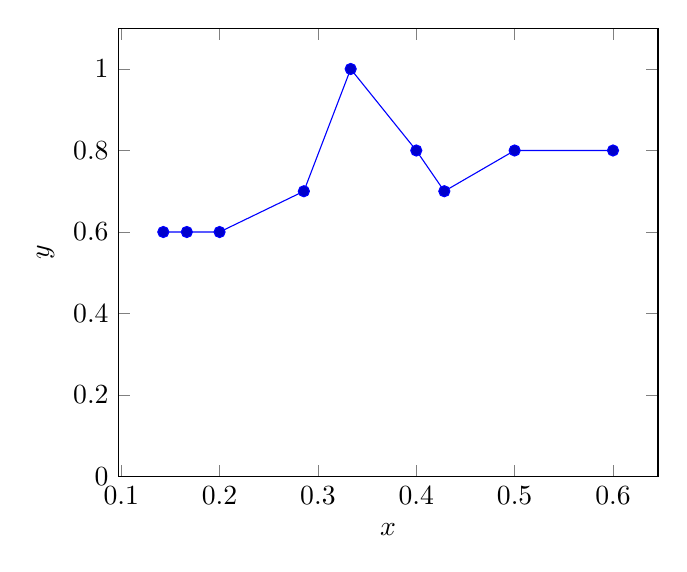
\begin{tikzpicture}
		\begin{axis}[
		  ymin=0,
		  xlabel=$x$,
		  ylabel=$y$,]
		  \addplot coordinates {(0.1428,0.6) (0.1667,0.6) (0.2,0.6) (0.2857,0.7) (0.3333,1.0) (0.4,0.8) (0.4285,0.7) (0.5,0.8) (0.6,0.8)};
		\end{axis}
	\end{tikzpicture}
    \caption{Геометрическая интерпретация $\tilde{O}=\tilde{N} \div \tilde{M}$}
    \label{fig:n_div_m}
\end{figure}

\subsection{Выводы}

В результате выполнения лабораторной работы были изучены теоретические основы по выполнению арифметических операций над нечеткими числами (сложение, вычитание, умножение, деление), а также закрепили теоретические знания решением практической задачи.

\end{document}
